\documentclass[../ClassicThesis.tex]{subfiles}

\newcount\colveccount
\newcommand*\colvec[1]{
        \global\colveccount#1
        \begin{pmatrix}
        \colvecnext
}
\def\colvecnext#1{
        #1
        \global\advance\colveccount-1
        \ifnum\colveccount>0
                \\
                \expandafter\colvecnext
        \else
                \end{pmatrix}
        \fi
}

\begin{document}

%************************************************
\chapter{Approximation}\label{ch:approximation}
% \secauthor{DS}
%************************************************

\newcommand\myNotes[1]{\textcolor{red}{#1}}


In this chapter we describe our methods to reduce the complexity of our data.

The pipeline step \emph{Simplification} provides a simplified version of the {\threedmodel} for all subsequent processing steps. The operation is called mesh simplification. This processing step serves two purposes: Removal of unwanted details and runtime improvement.

The implemented mesh simplification is called vertex welding. It is also reused in other processing steps of our software to remove unnecessary vertices.

Furthermore we eliminate obsolete vertices during shape generation with point on line removal.


\section{Mesh Simplification}


Mesh simplification reduces the complexity of a {\threedmodel} by decreasing the amount of vertices and faces. In this process the original object gets approximated with less information. While doing so the differences between the processing results of an original and an approximated object are kept as low as possible.

Our mesh simplification tackles three issues:

\paragraph*{Processing Time}

After the model is loaded and stored we decrease its complexity to speed up following processing tasks. Every pipeline step benefits from this mesh simplification because of the reduced data they are working on which implicates a much faster pipeline runtime.

\paragraph*{Abstraction}

Furthermore we eliminate beveled edges that are not functional but created by 3D-modeling software because of aesthetic reasons. These can be removed since they do not serve any functionality and raise the complexity for conversion. The vertex welding approach gives us the needed shape abstraction to extract tiny details and minor curvatures we do not want to reproduce.

\paragraph*{Elimination of redundant information created by our processing pipeline}

The algorithm can be reused in further processing to ensure unambiguous vertices that may occur due to rounding differences during transformations.


The used technique is known as vertex welding in computer graphics: We merge two or more vertices that lie in a specified distance to each other. Then the mesh contains fewer vertices. As a consequence of the smaller vertex set, thin faces no longer consist of three distinct vertices: Two nearby vertices are just represented by one vertex and the face gets deleted.

To illustrate the method the {\threedmodel} Stanford Bunny shown in Figure \ref{fig:origBunny} is simplified with an unusually high welding distance of 10mm in Figure \ref{fig:10mmBunny}. The images display each face with a different color to visualize the resulting face set. The loaded model consists of 8662 faces while the simplified bunny is reduced to 616 faces. Note, how smaller details like eyes and ears get lost with higher welding distance while the overall shape still remains. For effect illustration the welding distance is higher than the actual distance for processing.

\begin{figure}
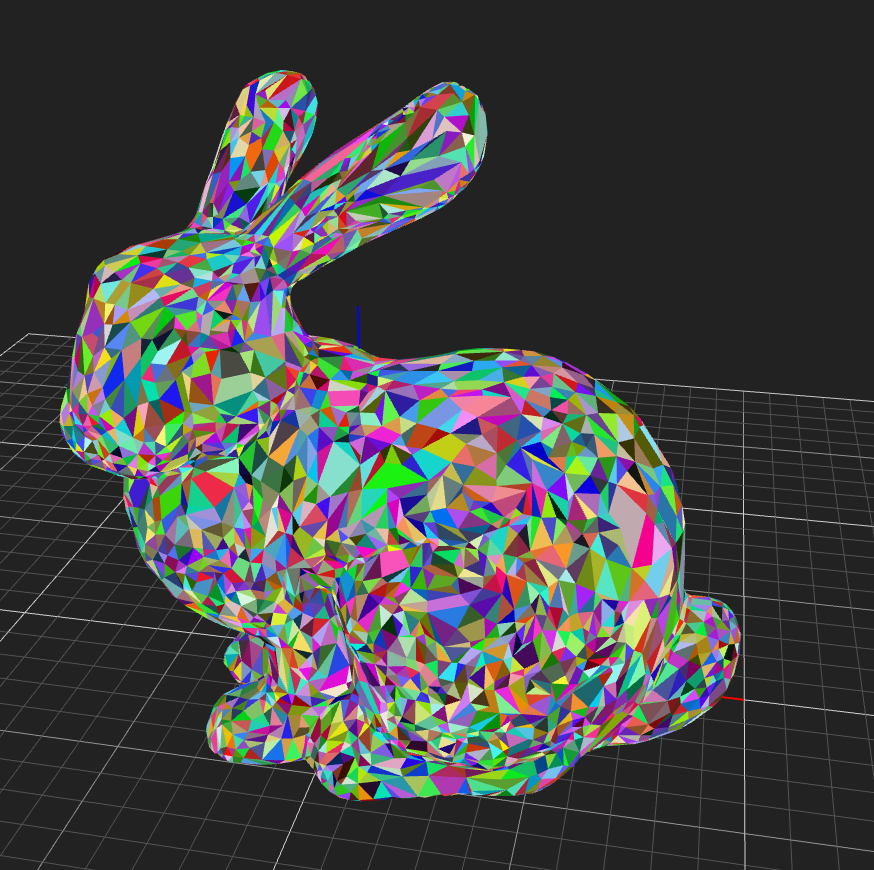
\includegraphics[width=0.8\columnwidth]{Images/04-approx-welding-rabbit-original.png}
\caption{Stanford Bunny with 8662 faces}
\label{fig:origBunny}
\end{figure}

\begin{figure}
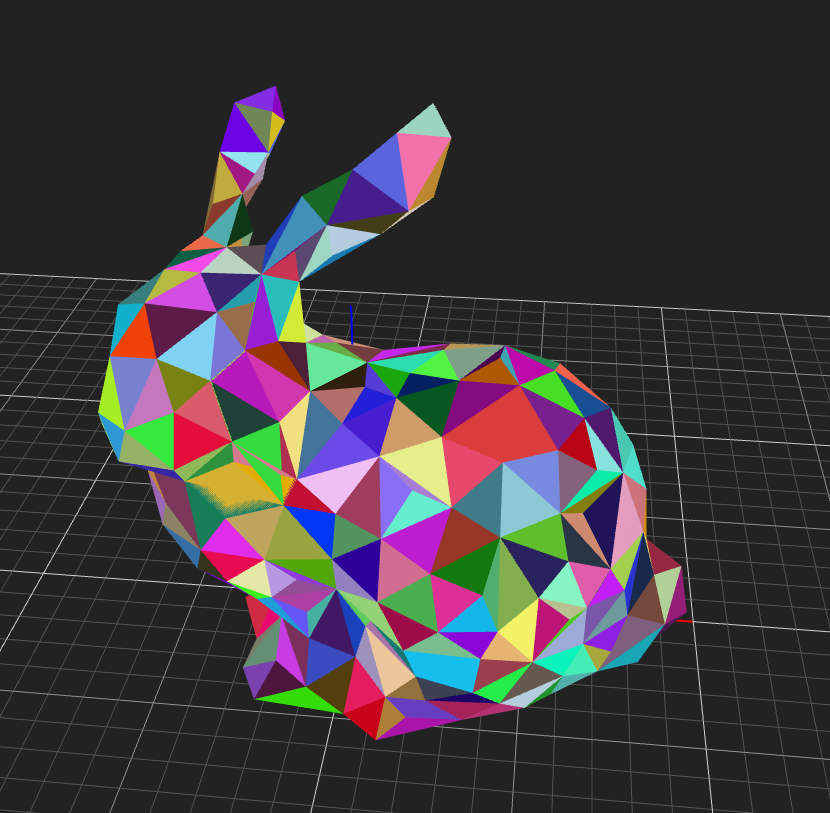
\includegraphics[width=0.8\columnwidth]{Images/04-approx-welding-rabbit-10mm.png}
\caption{Simplified Stanford Bunny with 616 faces. Applied welding distance: 10mm}
\label{fig:10mmBunny}
\end{figure}




\subsection{Vertex Welding}
\label{sec:vertex_welding}

% Überblick

% 2 Modi -> preprocessed, first come


% Algorithmus erklären...


% Hase

% Beveled edges



Vertex Welding merges vertices and works as shown in Figure \ref{fig:vertex_welding}:

A set of triangles is given. We choose a welding distance so points that lie further away of each other will not get merged. This is also the maximum distance a merged vertex can be away from its original position. Therefore it describes the variance of input and resulting vertex set.

For each cluster of vertices that gets merged, a new vertex is created which is typically in the middle of all corresponding points. The original vertices are replaced by this new one in each triangle.

In case a triangle $ABC$ has two points $A$ and $b$ in the same merge cluster, both get replaced by the new vertex $V$. As a result the triangle consists of the points $VVC$ while it does not contain three distinct vertices anymore - it is a line. If all three of its points lie in a cluster the outcome triangle $VVV$ is a single point. In these cases the triangle gets deleted. The initial area of these deleted triangles is now covered by its adjacent triangles.

The result is an approximation of the input with fewer vertices and faces while the maximum variance equals the specified welding distance. As illustrated in Figure \ref{fig:vertex_welding}, the resulting shape can also completely equal the original one without any differences: Only vertices inside the rectangle got merged which does not affect the outline of the object.



\begin{figure}
\includegraphics[width=0.8\columnwidth]{Images/04-approx-welding-overview2.png}
\caption{Vertex Welding}
\label{fig:vertex_welding}
\end{figure}

\subsubsection{How the vertex algorithm is used in our software}

For each welding application a new instance of \emph{VertexWelding} is created with the desired welding distance. Then, the data can be preprocessed before the actual welding which provides the best possible result. Each vertex is then replaced by the \emph{VertexWelding} vertices. The points can be merged without preprocessing in case it is not needed, e.g. while using very small welding distances.

\emph{VertexWelding} provides five functions:

\subsubsection*{preProcessModel}

preprocesses the given meshlib model.

\subsubsection*{preProcessVertices}

preprocesses the given array of vertices. A Vertex may be any object containing \emph{x}, \emph{y} and \emph{z} values.

\subsubsection*{preProcessVertex}

preprocesses the given vertex which may be any object containing \emph{x}, \emph{y} and \emph{z} values.

\subsubsection*{getCorrespondingVertex}

returns a new vertex based on the given one. This function is called for replacing each point of an object.

\subsubsection*{replaceVerticesAndDeleteNonTriangularFaces}

handles the welding process for the given meshlib model: It replaces all vertices and deletes triangles that are not needed any more.


So a set of vertices is welded by calling \emph{preprocessVertices}, iterating over all points and replacing them with the vertex from \emph{getCorrespondingVertex} or just replacing them without preprocessing.


\subsubsection{Implementation}

\emph{VertexWelding} builds a list of weighted vertices during preprocessing. All original points are replaced with these \emph{weightedVertices} during the welding process so this list contains all vertices that end up in the resulting dataset.

During list setup each new vertex is either merged with an existing \emph{weightedVertex} or added to the list. Therefore all original vertices are represented by a \emph{weightedVertex}. A \emph{WeightedVertex} saves the number of represented points to merge new vertices correspondingly as shown in Figure \ref{fig:weightedVertex}.

In this figure point 1 is a \emph{weightedVertex} with $weight = 2 $. Point 2 is the next vertex to be preprocessed and is within welding distance to point 1. Therefore point 2 is merged with point 1. The resulting point 3 lies between point 1 and 2. Since point 1 has $ weight = 2 $ the distance between point 3 and 1 is half the distance between point 3 and 2.

\begin{figure}
\includegraphics[width=0.4\columnwidth]{Images/04-approx-WeightedVertex.png}
\caption{Point 3 is the result of merging point 1 and 2. Point 1 is a weightedVertex with weight = 2}
\label{fig:weightedVertex}
\end{figure}

After preprocessing all points of a given set have to be replaced while \emph{getCorrespondingVertex} returns the respective vertex for each requested point.

In case a point is requested without preprocessing \emph{VertexWelding} builds its list without putting the new vertex in between the merged points, but picks the first one as representative for all following.




\paragraph{Preprocessing}

Preprocessing is done with one of the following methods:

\begin{description}
    \item preProcessModel
    \item preProcessVertices
    \item preProcessVertex
\end{description}

They iterate over the weighted vertex list and weld the new vertex with an existing one if they are in welding distance. The vertex is just added to the list, if it was not merged after complete iteration. This process is explained by listing \ref{lst:weldingLoop} which shows simplified pseudo code.

\begin{listing}[!h]
\centering
\begin{minted}[
linenos, breaklines
]{coffeescript}
preProcessVertex (newVertex) ->
    for wv in weightedVertices
        if wv.isInWeldingDistanceTo(newVertex)
            wv.merge(newVertex)
            return
    weightedVertices.push( new WeightedVertex(newVertex) )
\end{minted}
\caption{Algorithm for preprocessing a new vertex}
\label{lst:weldingLoop}
\end{listing}

Merging is done by adding a fraction of the vector between \emph{WeightedVertex} and new vertex. The fraction is based on the weight of the \emph{WeightedVertex} which is the amount of already welded vertices.

A \emph{WeightedVertex} $\vec{v}_{weighted}$ is instanced with weight $w = 1$. When a point $\vec{v}_{new}$ is added, weight gets increased and the new coordinates are computed:

$ w = w + 1 $

$ \vec{v}_{weighted} = \vec{v}_{weighted} + \frac{\vec{v}_{new} - \vec{v}_{weighted}}{w}$


\paragraph{Vertex Replacement}

The actual vertex replacement is done manually for each point with \emph{getCorrespondingVertex}, meaning \emph{VertexWelding} just provides the new vertices and does not replace the old ones. It iterates over the weighted vertex list and returns a point if it is in welding distance. After iteration it adds the vertex to its weighted vertex list in case there was no corresponding one. This automatically handles welding without preprocessing: Each passed vertex is added to the list as long there is no vertex in welding distance yet. Therefore the first vertex serves as representant for all following ones that lie nearby.

A complete model can be handled with \emph{replaceVerticesAndDeleteNonTriangularFaces}. It takes a \emph{meshlib} model and iterates over all faces. Each of the three points gets replaced and a face gets deleted if its points are not distinct anymore.




\subsection{Simplification Pipelinestep}

After the pipeline step \emph{ModelStorage} saved the unmodified {\threedmodel} \emph{Simplification} provides a simplified version for all subsequent processing steps. It is directly followed by \emph{MeshSetup} and \emph{CoplanarFaces} which analyses the given mesh to combine multiple faces.

This processing step serves two purposes: Removal of unwanted details and runtime improvement. Due to the capability of representing details with stacked plates, \emph{Simplification} is not run in the fabrication method \emph{StackedPlates}.

\subsubsection{Details with stacked plates}

If sliced in an advantageous direction tiny details of a {\threedmodel} can be obtained with stacked plates. These details may be textures or bump maps like an engraving or a rough surface.

In general \emph{Simplification} removes such details as shown in Figure \ref{fig:3mmMakerbotMake}. With a welding distance of 3mm the result is a smooth surface while the original model shown in Figure \ref{fig:origMakerbotMake} contains the text 'Make:'.

To simplify a model without loosing such a text is not possible with the implemented vertex welding due to the nature of these texts: The labeled surface differs barely from a smooth surface. Therefore the vertices are so close to each other that welding will occur with every chosen welding distance. To obtain those texts the algorithm has to know areas where it must not weld. If tried to outline the text with a smaller welding distance there will always be some kind of artifacts: missing or degenerated letters like in Figure \ref{fig:08mmMakerbotMake}.

In order to be able to represent such texts with stacked plates \emph{Simplification} is not run in the fabrication method \emph{StackedPlates}.


\begin{figure}

\includegraphics[width=0.8\columnwidth]{Images/04-approx-welding-make-unwelded.png}
\caption{Original Makerbot letters}
\label{fig:origMakerbotMake}
\end{figure}

\begin{figure}
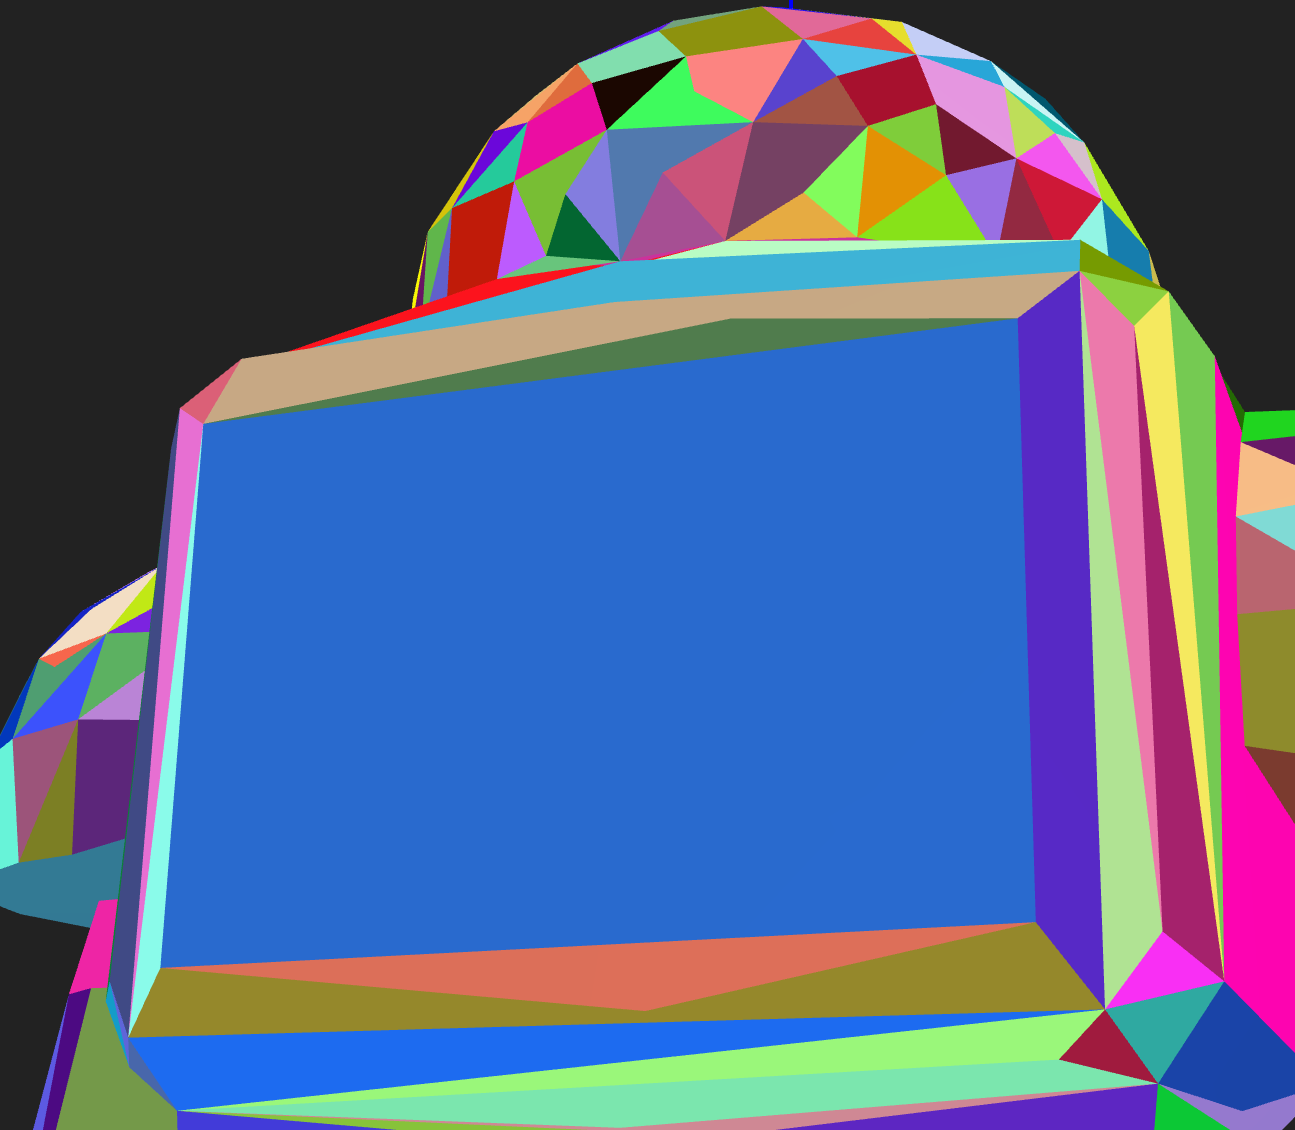
\includegraphics[width=0.8\columnwidth]{Images/04-approx-welding-make-3mm.png}
\caption{Simplified Makerbot with welding distance 3mm - letters completely removed}
\label{fig:3mmMakerbotMake}
\end{figure}

\begin{figure}
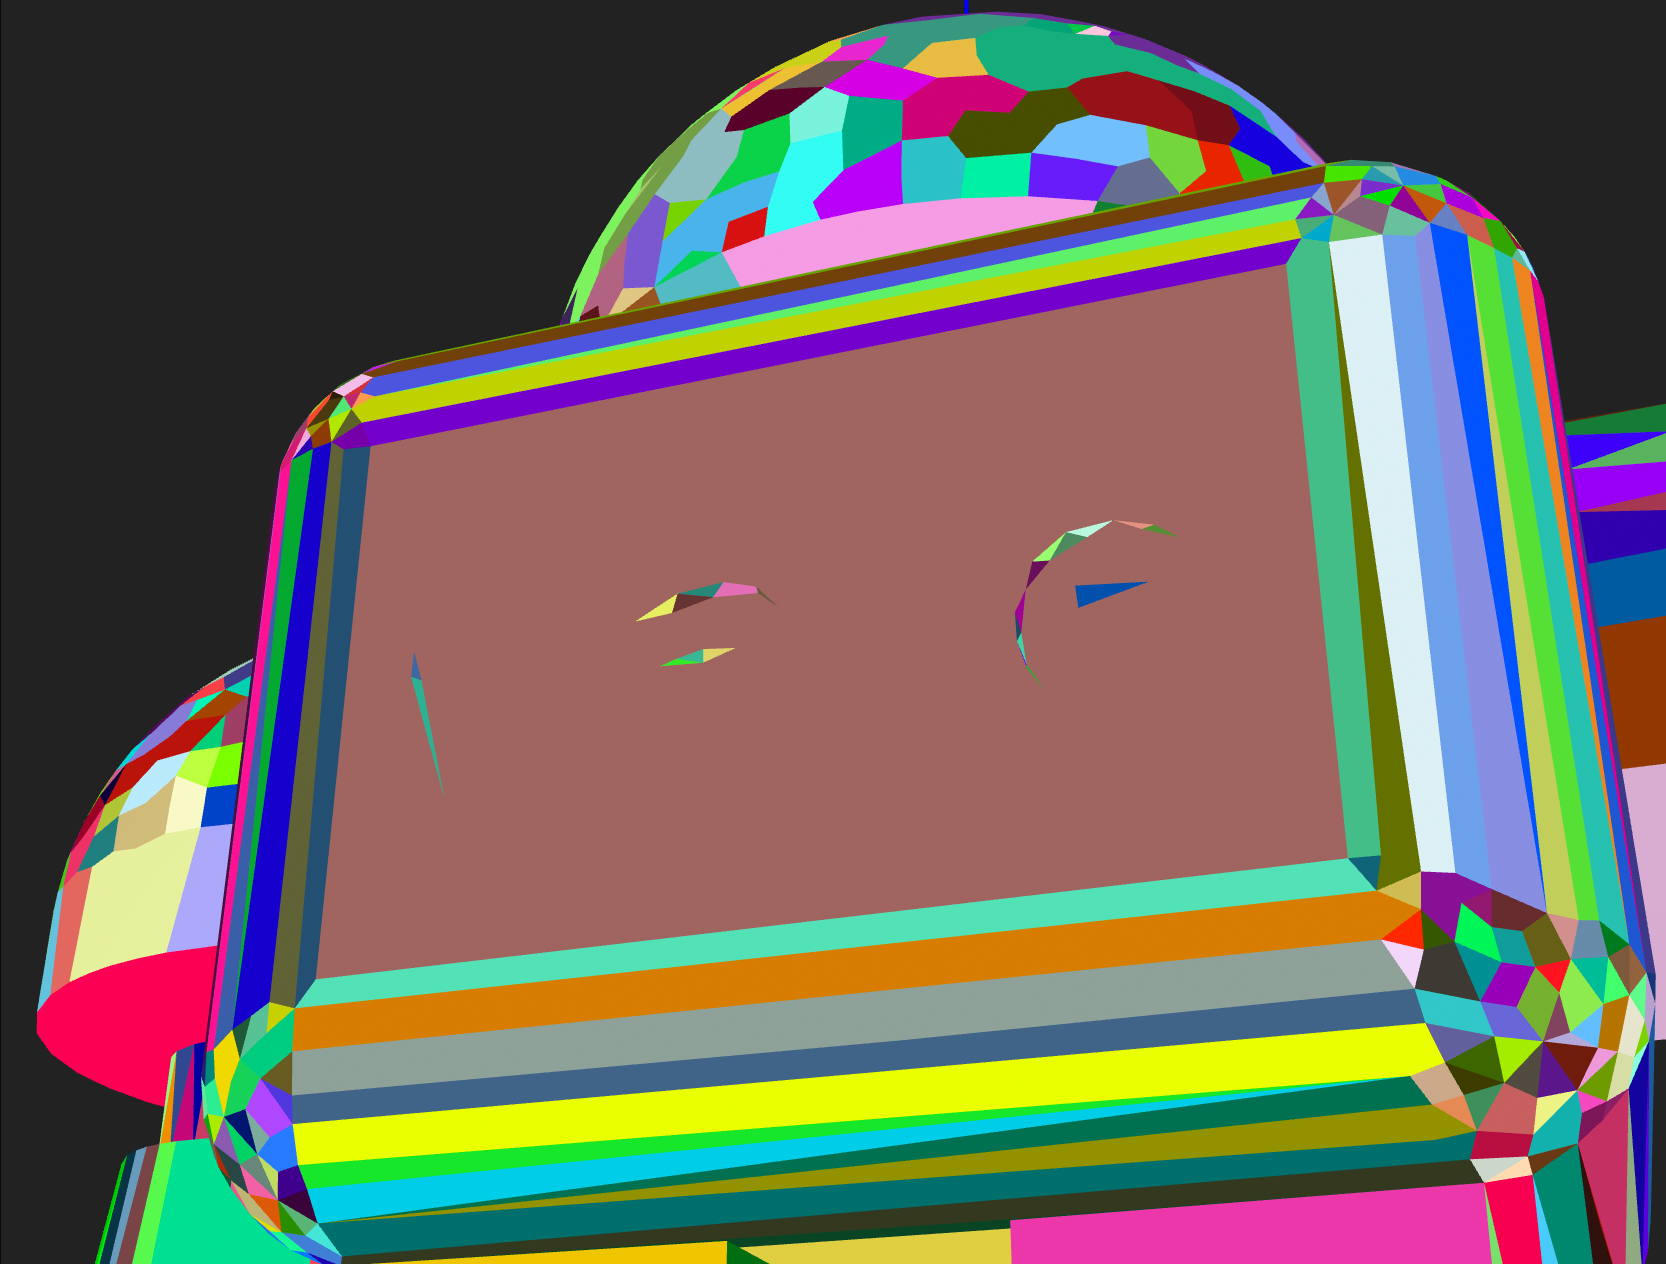
\includegraphics[width=0.8\columnwidth]{Images/04-approx-welding-make-0_8mm.png}
\caption{Simplified Makerbot with welding distance 0.8mm - artifacts}
\label{fig:08mmMakerbotMake}
\end{figure}

\subsubsection{Unwanted Details}

Most 3D editors offer to prettify objects by using curvatures instead of sharp edges. This can be done in various nuances to determine the smoothness of the curve.

Obviously it is much easier to reproduce two connected plates without a beveled edge in the pipeline step \emph{InherentPlates}. Since these curvatures are just for aesthetic reasons we revert the rounding without any loss of functionality.

Figure \ref{fig:beveled} shows three beveled cubes where the edge is subdivided into one, two and ten parts. All three result in the cube with straight edges after the \emph{Simplification}. The granularity of the created beveled edge does not make any difference for the outcome:
The higher the number of parts the denser the vertices while the absolute distance between start and end of a beveled edge remains the same. Therefore all vertices in this area get merged to the desired point independently from the edge segmentation.

In addition all sorts of surface modification like engravings and small attachments get removed which simplifies the plate recognition. In Figure \ref{fig:extruded_details} there is text on top of the actual surface and in Figure \ref{fig:pushed_in_details} there is text pushed into the surface while both text is removed in the resulting object.


\begin{figure}
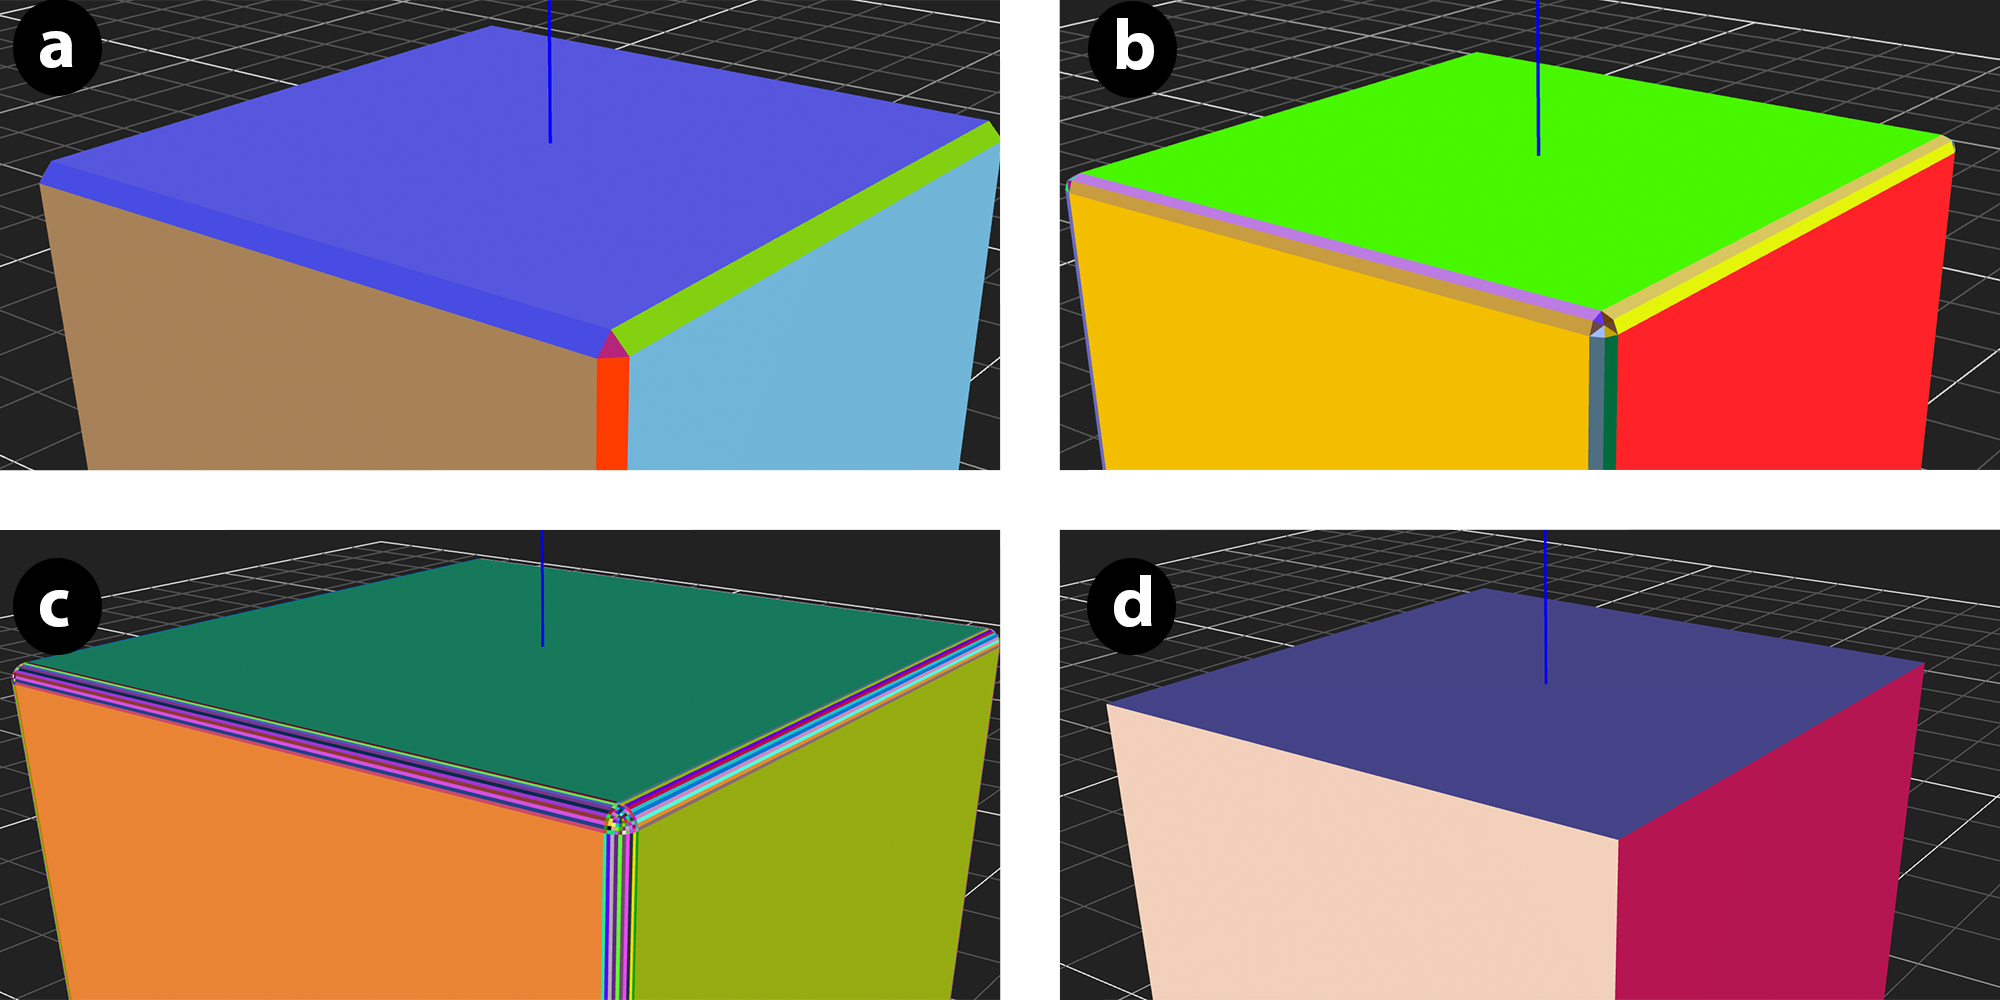
\includegraphics[width=1.0\columnwidth]{Images/04-approx-welding-beveled-2.png}
\caption{Beveled cube a) with 1 subdivision, b) with 2 subdivisions, c) with 10 subdivisions and their resulting cube d) without beveled edges}
\label{fig:beveled}
\end{figure}

\begin{figure}
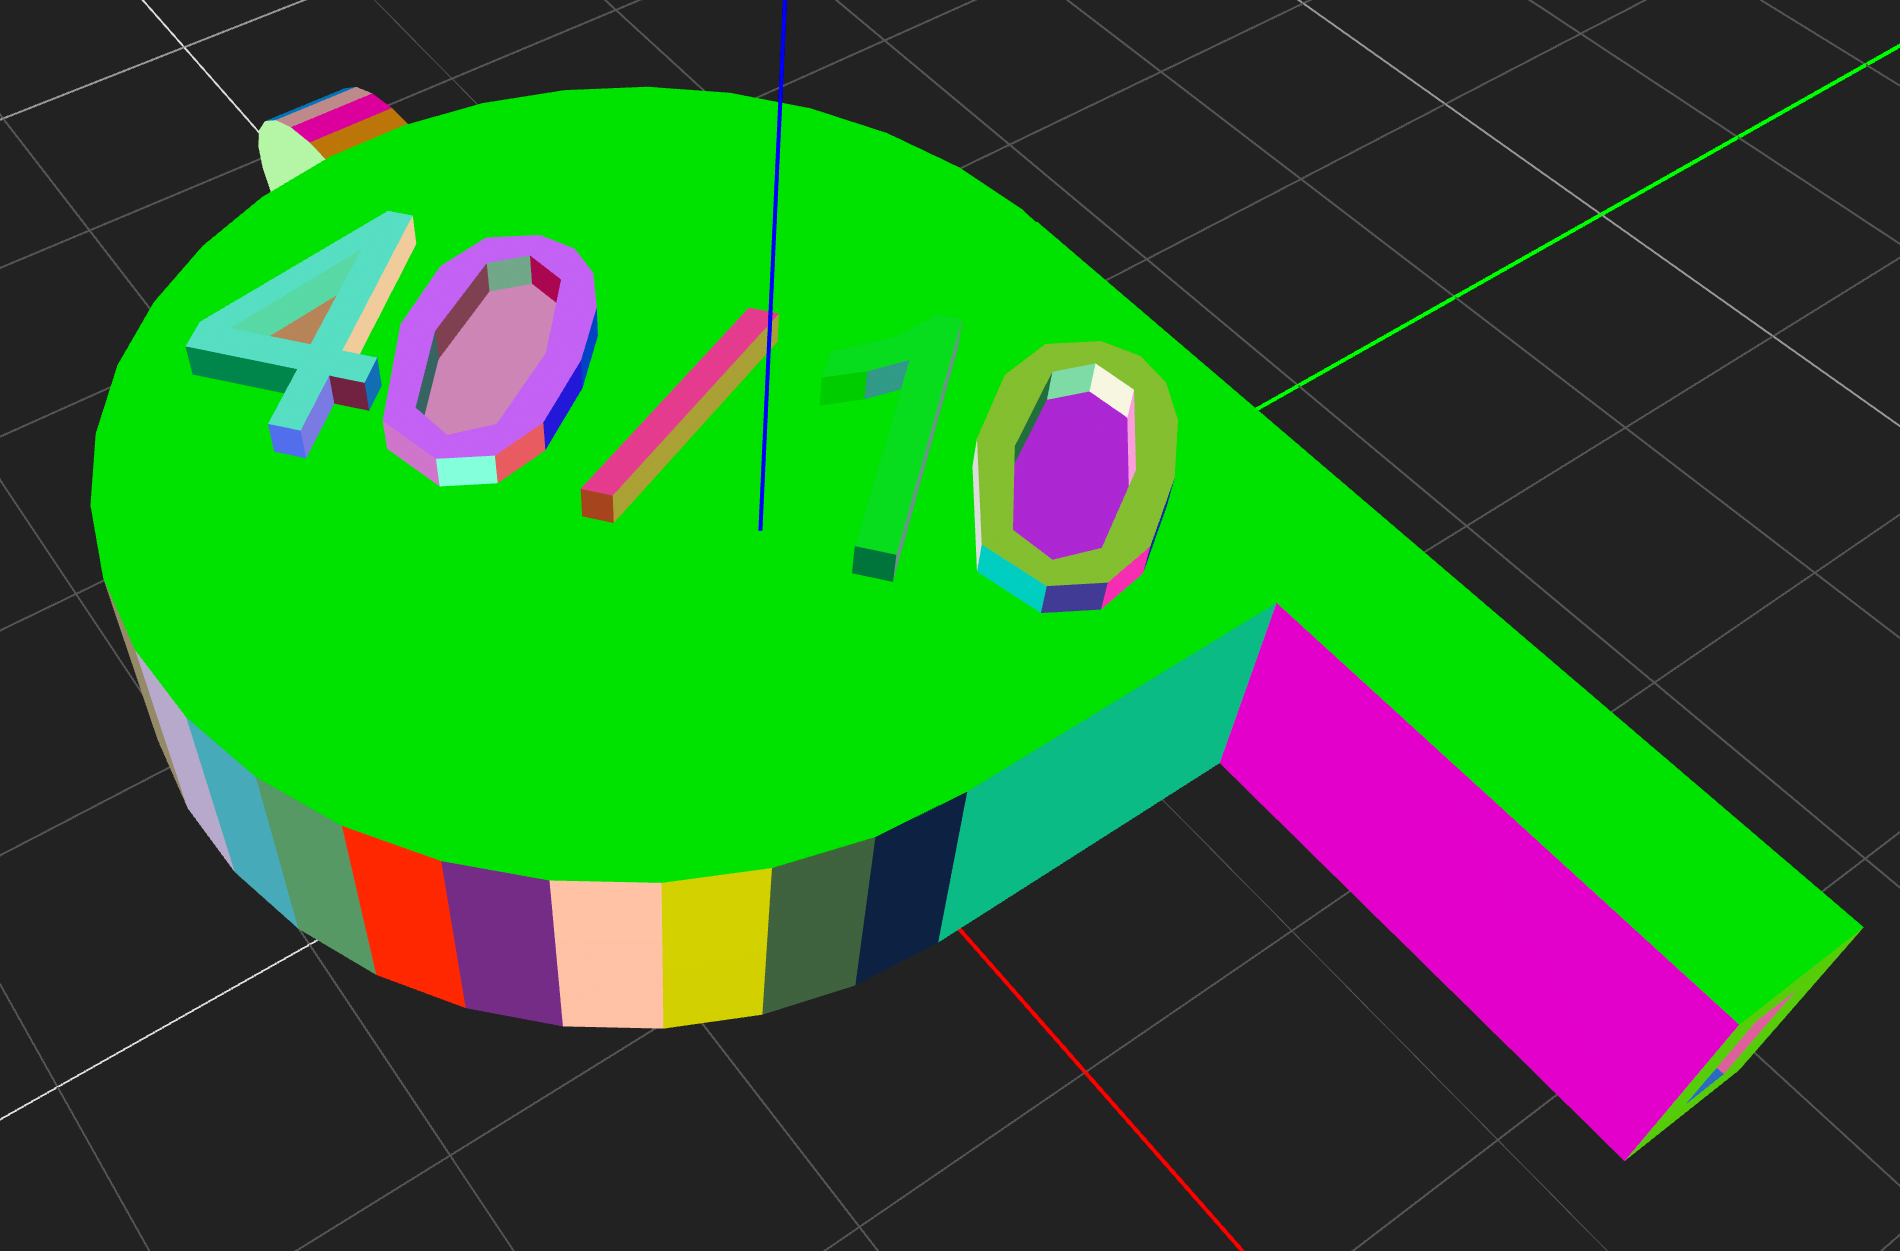
\includegraphics[width=0.5\columnwidth]{Images/04-approx-welding-beveled-extruded.png}
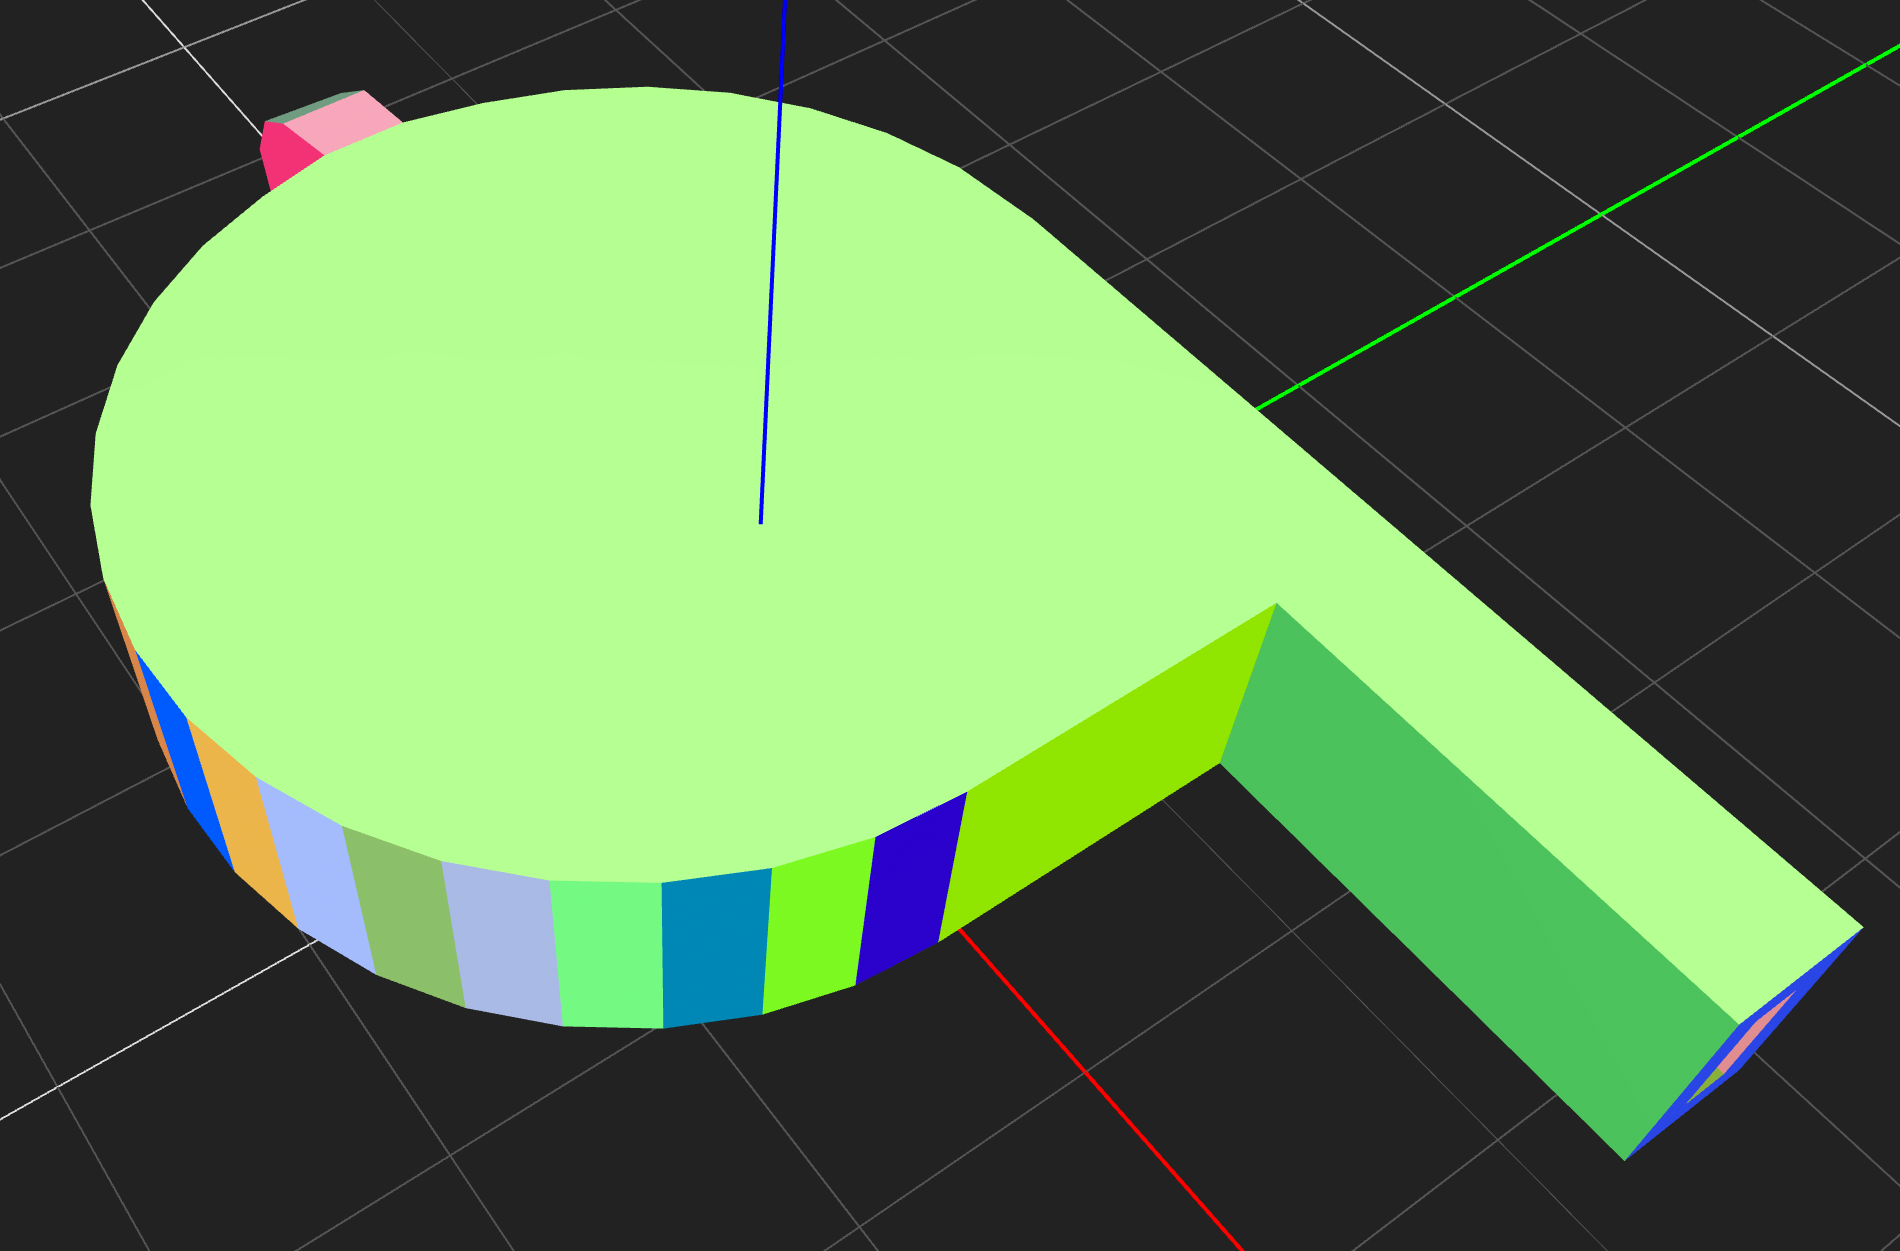
\includegraphics[width=0.5\columnwidth]{Images/04-approx-welding-beveled-extruded-result.png}
\caption{Extruded details get removed}
\label{fig:extruded_details}
\end{figure}

\begin{figure}
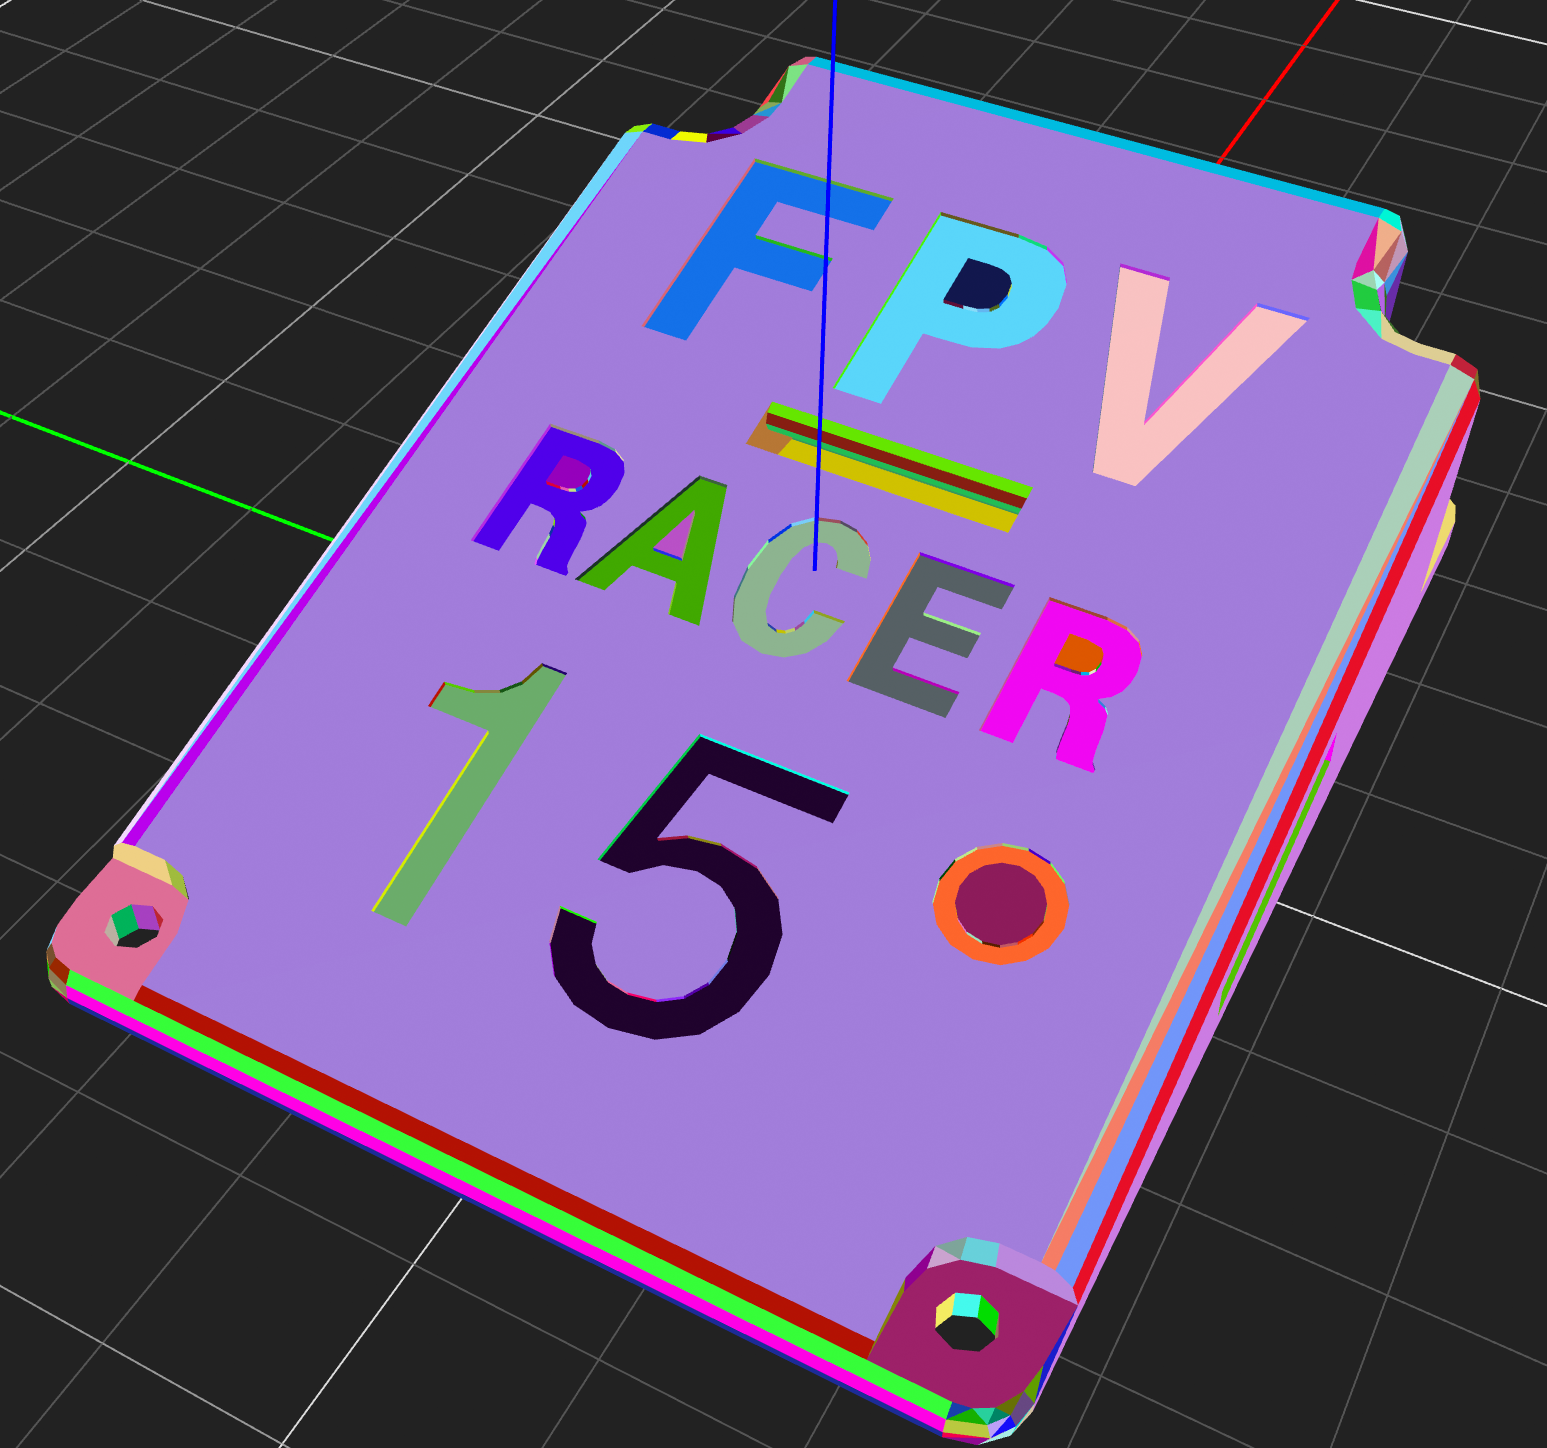
\includegraphics[width=0.5\columnwidth]{Images/04-approx-welding-pushedIn.png}
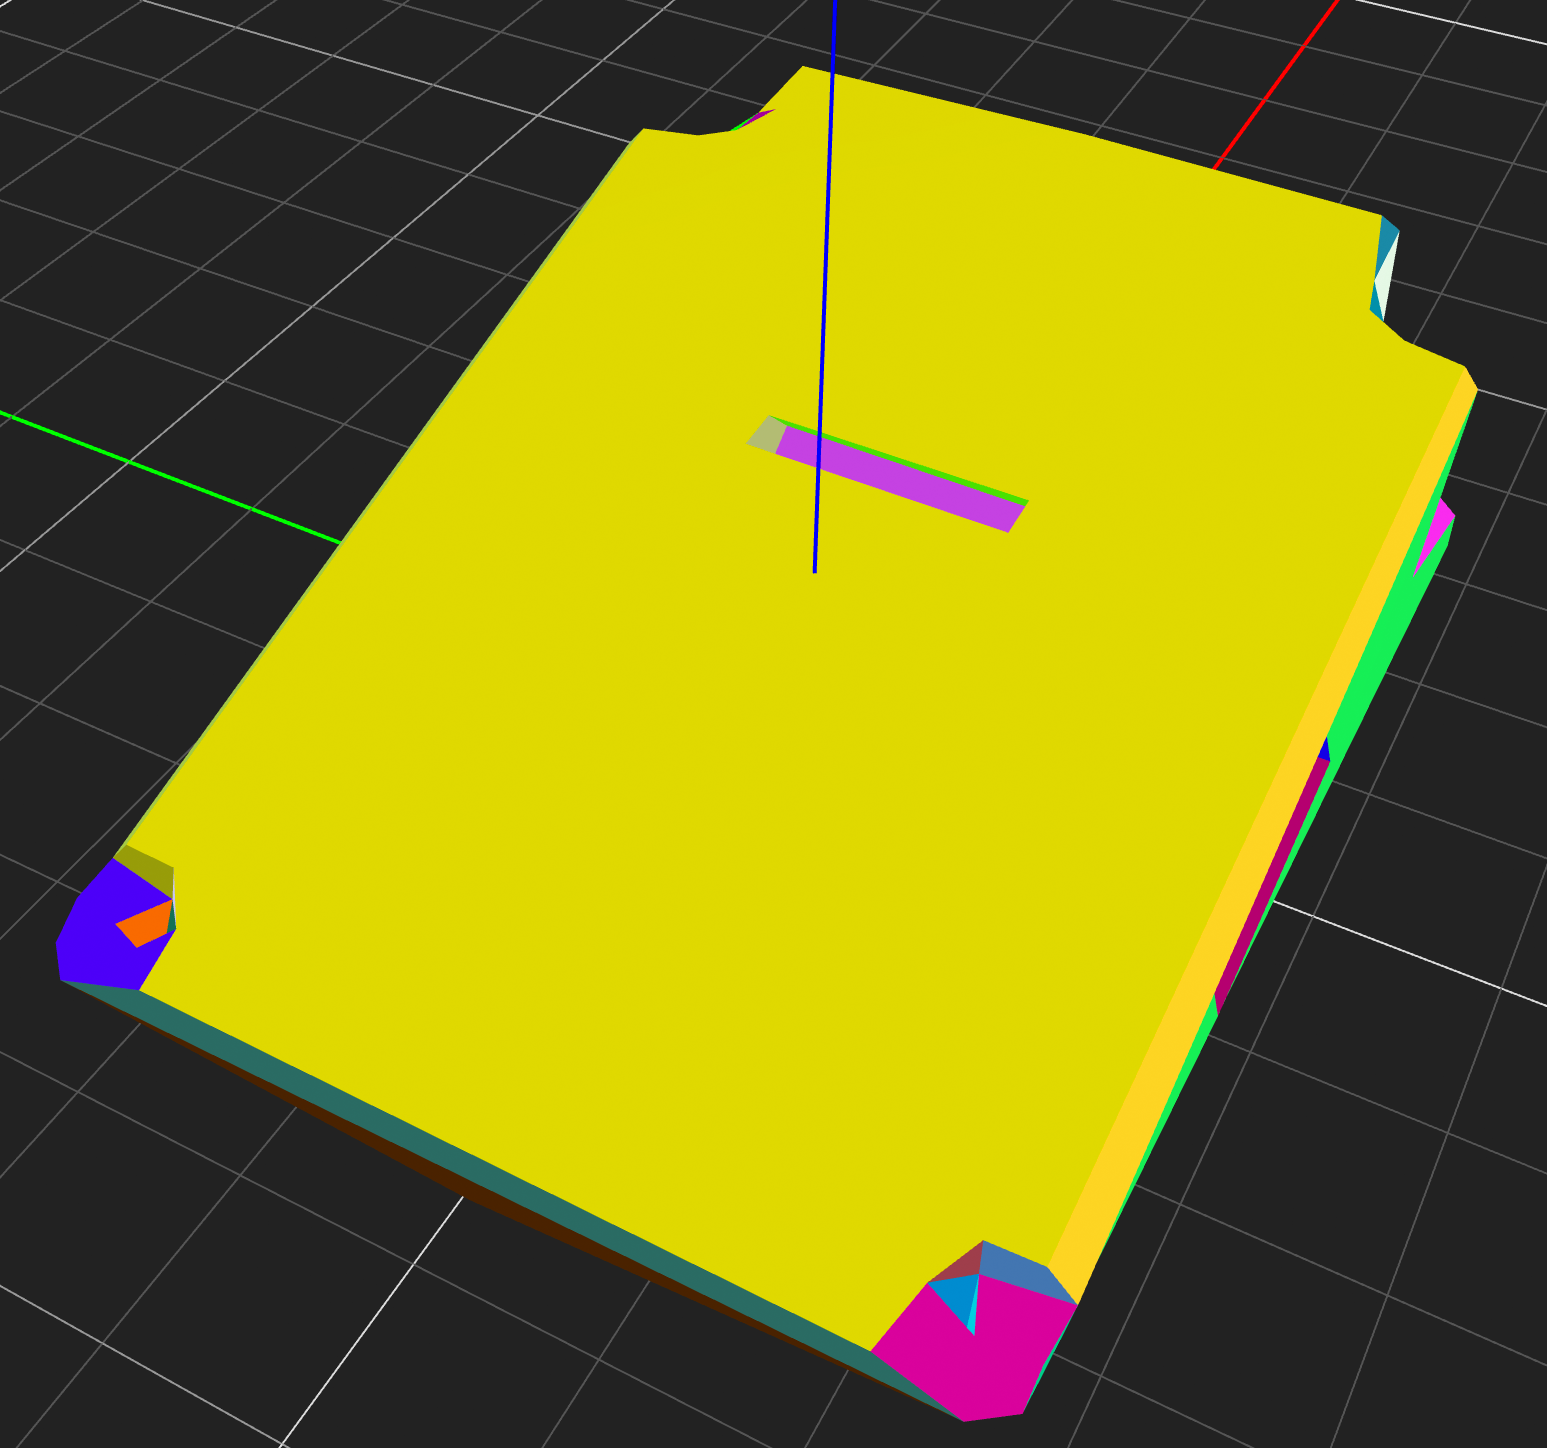
\includegraphics[width=0.5\columnwidth]{Images/04-approx-welding-pushedIn-result.png}
\caption{Pushed in details get removed}
\label{fig:pushed_in_details}
\end{figure}


\subsubsection{Process}

The pipeline step clones the model due to our immutable state approach so the original model can be accessed at any point in time. The immutable state approach is described in chapter \ref{ch:architecture} Architecture.


\paragraph{Welding Distance}

The welding distance is calculated based on the dimensions of the {\threedmodel}. Very small objects will not be welded at all and the welding distance increases with bigger models.

For most models a welding distance of 2mm is applied which removes all beveled edges created by common editors like Blender\footnote{https://www.blender.org}. Due to the nature of beveled edges all beveling methods only modify small areas around corners which results in dense vertices that get merged by our vertex welding.

The user can modify the welding distance in the UI element shown in Figure \ref{fig:weldingUI}. This is useful if the user only needs a rough approximation and does not care about small details so a greater welding distance can be chosen.

\begin{figure}
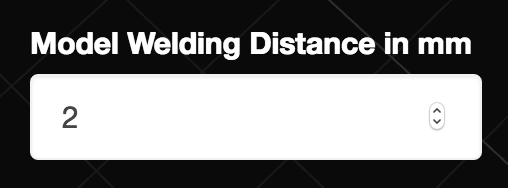
\includegraphics[width=0.5\columnwidth]{Images/04-approx-weldingUI.png}
\caption{Vertex Welding UI Element}
\label{fig:weldingUI}
\end{figure}



\paragraph{Welding}

At first all vertices get preprocessed by the welding algorithm to create the vertex lookup-table. After that the model is passed to \emph{VertexWelding} which iterates over all faces to replace its vertices with their corresponding vertex from the preprocessed table. Meanwhile it checks for invalid faces and deletes them.

\paragraph{Provided Model}

After the actual vertex welding the {\threedmodel} is checked for an empty face set which might occur if the user picked a large welding distance. In this case the stored and unmodified mesh is returned in order to run the rest of the pipeline. The user gets reminded to pick a better welding distance.

The mesh preparation itself is extracted into another pipeline step: \emph{MeshSetup}. It takes the simplified {\threedmodel} and makes it ready for all further processing: face vertex mesh building, normal calculation and mesh indexing.



\subsection{Reusage for redundant information elimination}

The algorithm can be reused in later processing steps. This is done for two reasons:

First a cluster of multiple points lying close together might not bring any additional usable information. So one single representative point of that cluster leads to the same result produced by our system. Therefore the data set can be simplified to improve its processing.

Second a set of points that were only one point in the first place. Different operations on a single vertex shared by multiple primitives lead to slightly different resulting vertices in each primitive. This happens because of floating point inaccuracies. Since these were actually just one point they get merged with our vertex welding.

For instance, this may occur during curve creation as described in chapter \ref{ch:curves} Curves where \emph{VertexWelder} is used to eliminate these point cluster. In general whenever a new data object is generated welding can be applied to ensure unambiguous points.





\subsection{Alternative Methods for Vertex Welding}

There are different ways of implementing vertex welding. The three other appropiate approaches are sorting vertices with an octree, via hashing or via binary space partitioning.

We chose our approach because it serves the simplification step with welding the complete {\threedmodel} as well as reusing it in later processing steps whenever we want to weld a data set. Therefore we do not have to implement different welding methods for various usages. Other implementations may not be applicable, may not serve all usages or will not bring any significant time improvement.

However, the welding can be split into different methods in future work if a runtime improvement is needed. Concretely the pipeline step \emph{simplification} will use an octree to speed up the model simplification and the remaining welding operations will be done with the current implementation.

\paragraph{Octree}

The space is discretised into blocks which dimensions equal the welding distance. At first all vertices are sort into these buckets. Then points are compared within each block along with its 26 surrounding ones and merged accordingly.

This would perform slightly faster for complete mesh simplification and slightly slower for fragmental welding of small vertex sets. Due to the vertex arrangement of most objects the number of comparisons would be lower and consequential the runtime too. On the opposite it performs slower for welding steps that take only a small amount of vertices: Most of them have to be compared so the space discretisation does not bring any advantages.

The implementation of a octree based welding is a bit more complex than the current implementation. We did not chose the octree variant since the current implementation runs in adequate runtime, was faster to code and easier to test.

\paragraph{Hashing}

Hashing is similar to the Octree approach and sorts vertices into a hash list. The sorting is based on a hash value computed by a hash function. This method is usually used if only identical points are merged instead of vertices that lie close to each other.

Due to the nature of hash functions it is easy to identify identical points since they have the same hash vale. Contrary, different points will not end up with the same hash value even if they should be welded in case we use a higher welding distance. Therefore hashing is not applicable to our system.

\paragraph{binary space partition}

Binary space partitioning discretises the space into parts similiar to an octree. It divides the space into unequal parts containing just one point instead of dividing the space into equal parts containing various number of points. Therefore the amount of point comparisons can be reduced which leads to a faster algorithm.

However, the runtime improvement is marginal compared to an octree and is more complicated to implement, test and maintain. Therefore binary space partitioning is not appropiate for our system.





\section{Point on Line Removal}

\emph{PointOnLineRemover} is used by the \emph{ShapesFinder} to delete unnecessary vertices and therefore reducing their complexity. It checks every \emph{EdgeLoop} of a found shape for vertices that lie on implicit lines given by other vertices as shown in figure \ref{fig:pointOnLine1}: Point 2 lies on the line between point 1 and 3 and gets deleted.

\begin{figure}
    \includegraphics[width=0.4\columnwidth]{Images/04-PointOnLine-1.png}
    \caption{point 2 gets deleted because it lies on the line between point 1 and 3}
    \label{fig:pointOnLine1}
\end{figure}

\emph{Shapes} may represent only a line or a point instead of a 2D-shape if they do not contain enough vertices. An \emph{EdgeLoop} gets deleted if it contains less than three vertices after point on line removal because it does not span an area any more. In case the contour of a \emph{shape} gets deleted the complete \emph{shape} is obsolete and gets deleted as well.

A threshold for the distance of a point to a line is given by the global config since minor deviations from the line are not relevant.

A simplified pseudo code version of the actual removal algorithm is shown in listing \ref{lst:pointOnLineRemovalAlgo}: \emph{getPreviousIndices()} returns the two previous indices that are not removed and \emph{isPreviousOnLine(index, prev, prevprev)} returns true if $ vertex_{prev}$ lies on the line between $vertex_{index}$ and $vertex_{prevprev}$. So we iterate over all vertices while deleting all its previous vertices until the previous is not on the line.

\begin{listing}[!h]
\centering
\begin{minted}[
linenos, breaklines
]{coffeescript}
for index in [0...vertices.length] when index not in removedIndices
    while true
        {prev, prevprev} = @getPreviousIndices(index)
        if @isPreviousOnLine(index, prev, prevprev)
            removedIndices.push(prev)
        else
            break
\end{minted}
\caption{Simplified point on line removal algorithm}
\label{lst:pointOnLineRemovalAlgo}
\end{listing}


When checking if a point lies on a line it is not sufficient to calculate the distance only as illustrated in figure \ref{fig:pointOnLine2}: Point 2 gets deleted in case point 3 lies within threshold distance to the line between point 1 and 2. But the actual point that should be deleted is obviously point 3 since it lies directly on the line between point 2 and 4.

Therefore it is needed to check if a point lies in between the points spanning the line and not outside. In figure \ref{fig:pointOnLine2} point 2 lies outside of the line between point 1 and 3. With this additional check the resulting triangle consist of the points 1, 2 and 4 as obviously desired.


\begin{figure}
    \includegraphics[width=0.6\columnwidth]{Images/04-PointOnLine-2.png}
    \caption{Point 3 gets deleted even if point 2 is within welding distance of the line between point 1 and 3. This is done because point 2 lies not in between point 1 and 3 but outside of them.}
    \label{fig:pointOnLine2}
\end{figure}




% \section{Remove Contained Plates - in Lukas Kapitel}
% % \secauthor{DS}

% \emph{RemoveContainedPlates} is executed after plate generation and removes unnecessary ones that appear with our software.

% There are two types of plates that get deleted: First as already described in the master thesis \emph{Platener} \cite{master-thesis} in section '4.4.4 Removing contained plates', small plates can be created that completely lie inside another plate. Second there may be parallel plates that lie inside each other. That occurs due to extrusion if the the 3D object is modeled with thicker blocks than the available material thickness.

% We iterate over all plates and compare them to all other plates. The comparison is based on their normals while further checks are not necessary most of the time because the normal check excludes most of them. Therefore the comparison is fast enough and the amount of comparisons must not be reduced with a different iteration algorithm.

% \subsection{Plate completely inside another}

% As described in the master thesis the algorithm may produce small plates that lie completely inside the actual modeled plate. These plates are orthogonal.

% So if two plates have orthogonal normals we check if one of them lies completely in the other and remove it.


% \subsection{Overlapping parallel plates}

% A 3D block can not be represented by one single plate if it is thicker than a plate. The software creates two plates instead. The resulting plates will overlap in case this block is thinner than those two plates together.

% So if two plates are parallel we compare their plane constants which specify the distance to the origin. In case the plane constants hint at overlap the actual \emph{EdgeLoops} are compared to identify intersections. In case they overlap one of the plates gets deleted.










% \section{Hole Detection - in Plates Kapitel}
% % \secauthor{DS}

% The pipeline step \emph{HoleDetection} is run after \emph{ShapesFinder} and categorises every \emph{edgeLoop} of each \emph{shape} either as outer contour or as hole. This is done by computing their areas and comparing them: The \emph{edgeLoop} with the biggest area is the outer contour and all others are holes.












% \chapter{Classifiers}
% \section{primitives}
% \subsection{Prism - Dimitri}
% % \secauthor{DS}

% A Prism is a base element for many other primitives which are characterized by two parallel shapes. Therefore a prism datastructure contains two shapes and the lateral surface as a set of primitives which are usually faces or shapes.

% To find the prisms all shapes have to be checked for parallelism. The comparison is based on normals which are sorted into buckets to speed up the process. The attached lateral surface can be identified by flood fill.

% \subsubsection{Bucket System}
% \label{sec:PrismBucketSystem}

% The surface normals $\vec{n}$ are sorted into buckets to reduce the amount of comparisons. Treating slightly different normals as equal considering a given threshold $\phi$ each bucket covers this angle. Therefore to check for similarity only normals within a bucket and the surounding ones have to be considered: The angle between two normals is always greater $\phi$ if their buckets are not neighbors. The corresponding bucket for a normal is determined by two values $\alpha$ and $\beta$. Their calculation is explained below.

% \begin{equation*}
%     \vec{n} = \colvec{3}{x}{y}{z}
% \end{equation*}


% All normals lie on the surface of the unit sphere because of their normalisation. Considering opposite normals as equal like planes with normals $(1,0,0)$ and $(-1,0,0)$ are parallel, all normals are transformed into a hemisphere as shown in Listing \ref{lst:_normalInHemisphere}: A normal is negated in case its $z$ value is negative.


% \begin{listing}[!h]
% \centering
% \begin{minted}[
% linenos
% ]{coffeescript}
% _normalInHemisphere: (normal) ->
%     if normal.z < 0
%         return normal.clone().negate()
%     else
%         return normal
% \end{minted}
% \caption{Normals are transformed into hemisphere}
% \label{lst:_normalInHemisphere}
% \end{listing}

% \begin{figure}
%     \includegraphics[width=0.9\columnwidth]{Images/PrismCl-Rings.png}
%     \caption{rings visualised from side}
%     \label{fig:rings_FromSide}
% \end{figure}

% \begin{figure}
%     \includegraphics[width=0.9\columnwidth]{Images/PrismCl-RingsFromTop.png}
%     \caption{rings visualised from top}
%     \label{fig:rings_FromTop}
% \end{figure}

% \begin{figure}
%     \includegraphics[width=0.4\columnwidth]{Images/PrismCl-RingAngle.png}
%     \caption{angle of a normal which is used for sorting it into a ring}
%     \label{fig:ringAngle}
% \end{figure}


% This hemisphere is separated into rings. Each ring covers the threshold angle $\phi$ in $z$-direction and is visualized in Figure \ref{fig:rings_FromSide} and Figure \ref{fig:rings_FromTop}. Each normal is sorted into a ring by its correlating angle $\alpha$ which is used to determine the ring index. It is proporional to its coordinates as demonstraded in Figure \ref{fig:ringAngle}: the angle between $\vec{n}$ and $(x,y,0)$:

% \begin{equation*}
% \begin{split}
%     \sin{\alpha} & = \frac{z}{ \sqrt{x^{2} + y^{2}} } \\
%     => \alpha  & = \arcsin{ \frac{z}{ \sqrt{x^{2} + y^{2}} } }
% \end{split}
% \end{equation*}


% The angle $\alpha$ is represented as a multiple of the threshold angle $\phi$ to get the actual ring index $I_{Ring}$:

% \begin{equation*}
%     I_{Ring} = \floor*{
%                     \arcsin{
%                         \frac{z}{ \sqrt{ x^{2} + y^{2} } }
%                     }
%                     / \phi
%                 }
% \end{equation*}

% The maximum angle is 90°. Consequently the maximum ring index $I_{MaxRing}$ is calculated as follows:

% \begin{equation*}
%     I_{MaxRing} = \floor*{
%                     \frac{\pi}{2}
%                     / \phi
%                   }
% \end{equation*}



% The angle in the middle of each ring ${\alpha}_{I_{Ring}}$ consequently depends on index and threshold:

% \begin{equation}
% \label{equ:AlphaIRing}
%     {\alpha}_{I_{Ring}} = (I_{Ring} + 0.5) * \phi \qquad \forall{ I_{Ring} \in [0, I_{MaxRing}] }
% \end{equation}



% Figure \ref{fig:middleZ} implies the calculation of the corresponding middle $z$ value $z_{I_{Ring}}$: We create a normal $\vec{a}_{I_{Ring}}$ with a fixed $y$ value of 0 that forms the angle ${\alpha}_{I_{Ring}}$ with the unit vector in x direction $\vec{v}_{x}$. Consequently all normals that lie in the middle of a ring ($\alpha = {\alpha}_{I_{Ring}}$) have the $z$ value $z_{I_{Ring}}$.

% \begin{figure}
%     \includegraphics[width=0.5\columnwidth]{Images/PrismCl-MiddleZ.png}
%     \caption{geometric visualization of the z value in the middle of a ring}
%     \label{fig:middleZ}
% \end{figure}

% \begin{equation}
% \label{equ:VecX}
%     \vec{v}_{x} = (1, 0, 0)
% \end{equation}

% \begin{equation}
% \begin{split}
%     \label{equ:VecA}
%     \vec{a}_{I_{Ring}} = (x_{a}, 0, z_{I_{Ring}}) \qquad  & \forall{ I_{Ring} \in [0, I_{MaxRing}] } \\
%     & with \vert \vec{a}_{I_{Ring}} \vert = 1
% \end{split}
% \end{equation}

% \begin{equation}
%     \label{equ:XA}
%     \cos{{\alpha}_{I_{Ring}}} = \frac{ \vec{v}_{x} * \vec{a}_{I_{Ring}} }{ \vert \vec{v}_{x} \vert * \vert \vec{a}_{I_{Ring}} \vert }
%     \stackrel{(\ref{equ:VecX}) + (\ref{equ:VecA})}{=} \vec{v}_{x} * \vec{a}_{I_{Ring}}
%     \stackrel{(\ref{equ:VecX}) + (\ref{equ:VecA})}{=} x_{a}
% \end{equation}

% \begin{equation}
% \label{equ:ZIRing}
% \begin{split}
%     1 & = \vert \vec{a}_{I_{Ring}} \vert \stackrel{(\ref{equ:VecA})}{=} \sqrt{ x_{a}^{2} + z_{I_{Ring}}^{2} } \\
%     => z_{I_{Ring}} & = \sqrt{1 - x_{a}^{2}}
%     \stackrel{(\ref{equ:XA})}{=} \sqrt{1 - cos^{2}{{\alpha}_{I_{Ring}}}}
% \end{split}
% \end{equation}


% Each ring is seperated into buckets which cover the threshold angle $\phi$ as shown in Figure \ref{fig:PrismCl-buckets}. Therefore the onto the xy-plane projected angle $\gamma$ needs to be calculated which differs from ring to ring. This is shown in Figure \ref{fig:projection} and leads to this calculation:

% \begin{figure}
%     \includegraphics[width=0.7\columnwidth]{Images/PrismCl-buckets.png}
%     \caption{buckets in a ring span the projected angle $\protect\gamma$ of the angle $\protect\phi$}
%     \label{fig:PrismCl-buckets}
% \end{figure}


% \begin{figure}
%     \includegraphics[width=1.0\columnwidth]{Images/PrismCl-Projection.png}
%     \caption{projection of the angle $\protect\phi$}
%     \label{fig:projection}
% \end{figure}


% $ \vec{a}_{I_{Ring}}' $ is the projection of $\vec{a}_{I_{Ring}} $:


% \begin{equation}
%     \label{equ:VecAStrich}
%     \vec{a}_{I_{Ring}}' = (x_{a}, 0)
% \end{equation}

% $ \vec{b}_{I_{Ring}} $ spans the threshold angle $\phi$ with $ \vec{a}_{I_{Ring}} $ and has the same $z$ value $z_{I_{Ring}}$:

% \begin{equation}
%     \vec{b}_{I_{Ring}} = (x_{b}, y_{b}, z_{I_{Ring}}) \qquad with | \vec{b}_{I_{Ring}}| = 1
%     \label{equ:VecB}
% \end{equation}

% The corresponding projected vector $ \vec{b}_{I_{Ring}}' $:

% \begin{equation}
%     \vec{b}_{I_{Ring}}' = (x_{b}, y_{b})
%     \label{equ:VecBStrich}
% \end{equation}

% Due to the mentioned conditions the coordinates of $ \vec{b}_{I_{Ring}} $ are calculated as follows:


% \begin{equation}
%     \label{equ:Projection1}
%     \cos{\phi} = \frac{\vec{a}_{I_{Ring}} * \vec{b}_{I_{Ring}}}{|\vec{a}| * |\vec{b}|} = \vec{a}_{I_{Ring}} * \vec{b}_{I_{Ring}} \stackrel{(\ref{equ:VecA}) + (\ref{equ:VecB})}{=} x_{a}_{I_{Ring}} * x_{b}_{I_{Ring}} + z_{I_{Ring}}^{2}
% \end{equation}

% \begin{equation}
%     \label{equ:XB}
%   (\ref{equ:Projection1}) => x_{b} = \frac{ \cos{\phi} - z_{I_{Ring}}^{2} }{ x_{a} }
% \end{equation}

% \begin{equation}
% \begin{split}
%     \label{equ:YpsilonB}
%     & 1 = |\vec{a}_{I_{Ring}}| = |\vec{b}_{I_{Ring}}| \\
%     & => \sqrt{ x_{a}^{2} + z_{I_{Ring}}^{2} } = \sqrt{ x_{b}^{2} + y_{b}^{2} + z_{I_{Ring}}^{2} } \\
%     & => y_{b} = \sqrt{ x_{a}^{2} - x_{b}^{2} }
% \end{split}
% \end{equation}


% The angle ${\gamma}_{I_{Ring}}$ which is used to separate a ring into buckets is calculated with the projected vectors $ \vec{a}_{I_{Ring}}' $ and $ \vec{b}_{I_{Ring}}' $ :

% \begin{equation}
% \begin{split}
%     \cos{{\gamma}_{I_{Ring}}}& = \frac{\vec{a}_{I_{Ring}}' * \vec{b}_{I_{Ring}}'}{|\vec{a}_{I_{Ring}}'| * |\vec{b}_{I_{Ring}}'|}
%     = \frac{ x_{a} * x_{b} }{ x_{a} * \sqrt{  x_{b}^{2} +  y_{b}^{2} } } \\
%     & \stackrel{(\ref{equ:YpsilonB})}{=} \frac{ x_{a} * x_{b} }{ x_{a} * \sqrt{  x_{b}^{2} - x_{b}^{2} +  x_{a}^{2} } }
%     = \frac{ x_{a} * x_{b} }{ x_{a} * x_{a} }
%     = \frac{ x_{b} }{ x_{a} } \\
%     & \stackrel{(\ref{equ:XB})}{=} \frac{ \cos{\phi} - z_{I_{Ring}}^{2} }{ x_{a}^{2} }
%     \stackrel{(\ref{equ:XA})}{=} \frac{ \cos{\phi} - z_{I_{Ring}}^{2} }{ \cos^{2}{{\alpha}_{I_{Ring}}} } \\
%     & \stackrel{(\ref{equ:ZIRing})}{=} \frac{ \cos{\phi} - ( 1 - cos^{2}{{\alpha}_{I_{Ring}}} ) }{ \cos^{2}{{\alpha}_{I_{Ring}}} }
%     = \frac{ \cos^{2}{{\alpha}_{I_{Ring}}} }{ \cos^{2}{{\alpha}_{I_{Ring}}} } + \frac{ \cos{\phi} - 1 }{ \cos^{2}{{\alpha}_{I_{Ring}}} } \\
%     & \stackrel{(\ref{equ:AlphaIRing})}{=} 1 + \frac{ \cos{\phi} - 1 }{ \cos^{2}{( (I_{Ring} + 0.5) * \phi )} } \\
%     => {\gamma}_{I_{Ring}} & = \arccos{( 1 + \frac{ \cos{\phi} - 1 }{ \cos^{2}{( (I_{Ring} + 0.5) * \phi )} } )}
% \end{split}
% \end{equation}


% The corresponding angle $ \beta $ of a normal $ \vec{n} $ is calculated with use of the unit vector in x direction $ \vec{v_{x}'} $. This angle needs to be adapted in case $ y < 0 $ since the maximum angle between two vectors is 180° and we want to cover a complete circle:

% \begin{equation}
% \begin{split}
%     \cos{\beta} & = \frac{\vec{n}' * \vec{v_{x}'}}{|\vec{n}'| * |\vec{v_{x}'}|} = \frac{x}{\sqrt{x^{2} + y^{2}}} \\
%     => \beta & = \begin{cases}
%         \arccos{ \frac{x}{\sqrt{x^{2} + y^{2}}} }, & y \geq 0 \\
%         2 \pi - \arccos{ \frac{x}{\sqrt{x^{2} + y^{2}}} }, & y < 0
%     \end{cases}
% \end{split}
% \end{equation}

% The angle $ \beta $ is represented as a multiple of the $ \gamma $ angle to get the bucket index $ I_{Bucket} $:

% \begin{equation}
%     I_{Bucket} = \floor{\frac{\beta}{ {\gamma}_{I_{Ring}} }}
% \end{equation}

% Consequently the maximum bucket index is calculated with the maximum angle of 360°:

% \begin{equation}
%     I_{MaxBucket} = \floor{\frac{2 \pi}{ {\gamma}_{I_{Ring}} }}
% \end{equation}



% \subsubsection{Implementation}

% The \emph{PrismClassifier} works on \emph{shapes} from the \emph{ClassifierGraph} and should also take account of \emph{planes} in future development. Therefore it depends on the \emph{PlaneClassifier}. It returns a set of \emph{prisms} and uses \emph{PrismShapeNormalsBuckets} to check shapes for parallelism. Its structure is represented in the class diagram figure \ref{fig:prismClassifierDiagram}.

% \begin{figure}
% 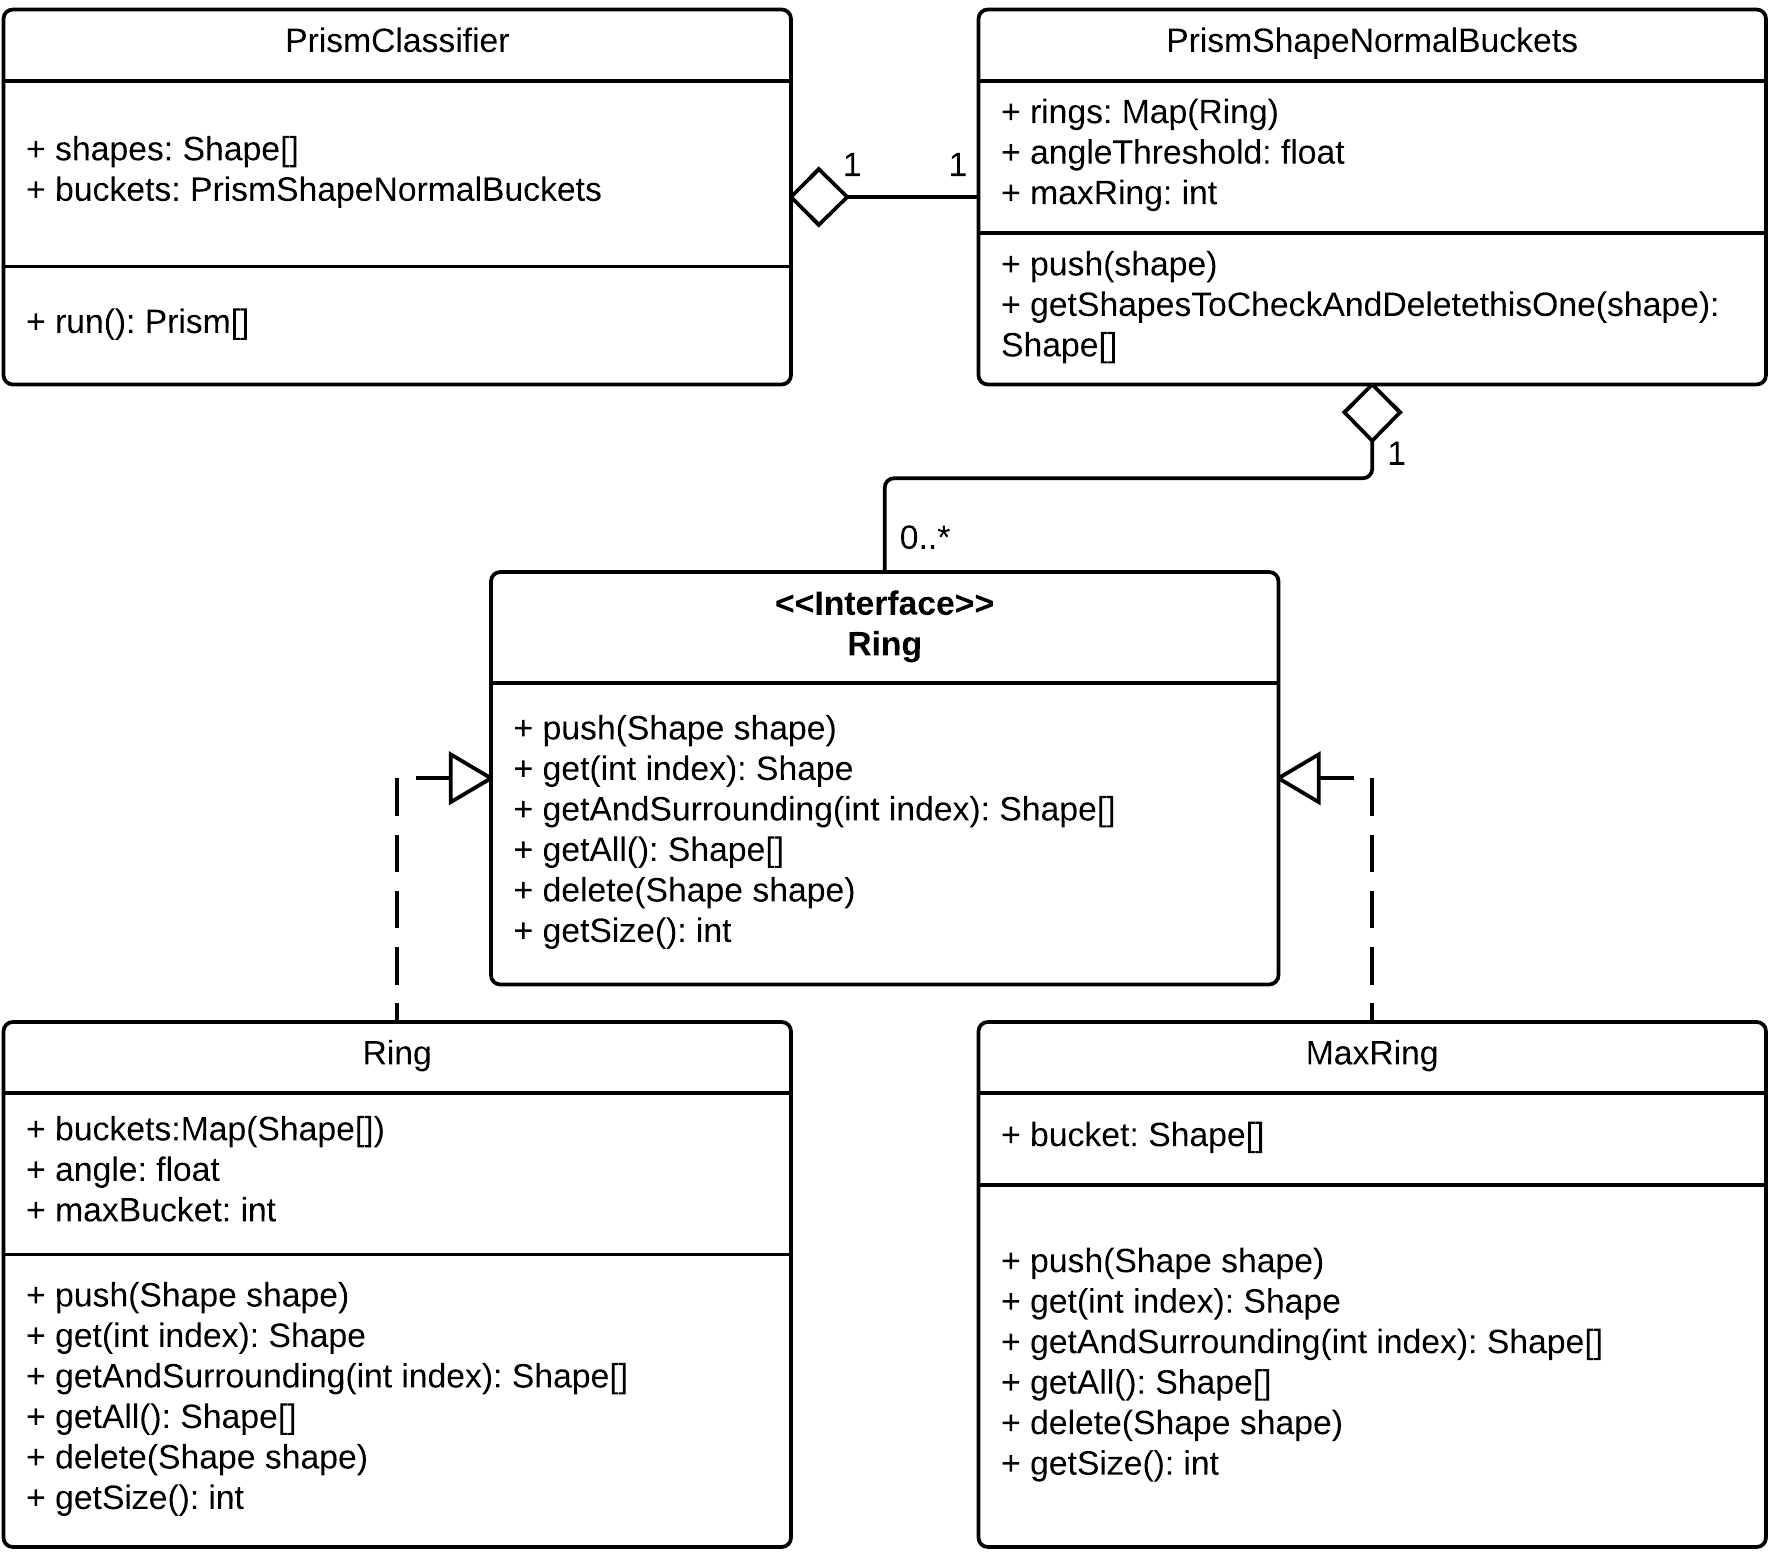
\includegraphics[width=1.0\columnwidth]{Images/04-prismClassifier.png}
% \caption{class diagram of the PrismClassifier}
% \label{fig:prismClassifierDiagram}
% \end{figure}

% \paragraph{PrismClassifier}

% \begin{listing}[!h]
% \centering
% \begin{minted}[
% linenos, breaklines
% ]{coffeescript}
% run: ->
%     return new Promise( (resolve) =>
%         buckets = new PrismShapeNormalsBuckets(_angleThreshold)

%         @_putIntoBuckets @shapes, buckets

%         prisms = @_detectPrisms @shapes, buckets

%         log.debug("PrismClassifier found " + prisms.length + " prisms")

%         resolve(prisms)
%     )
% \end{minted}
% \caption{run method of the PrismClassifier}
% \label{lst:PrismClassifierRun}
% \end{listing}

% Listing \ref{lst:PrismClassifierRun} shows the implementation of the \emph{PrismClassifier} run method:

% At first the normal buckets are initialised with an angle threshold as described in section \emph{Bucket System}. These values are stored in the global config with \emph{\_angleThreshold} $ = 0.15 $  ( = 8.6\textdegree, previously labeled $\phi$) so shapes with an angle  of 8.6\textdegree \hspace{1pt} will be considered parallel.

% Then all shapes are put into the corresponding buckets. This is done by iterating over all shapes and passing them to the bucket system which handles the classification on its own.

% Next we iterate over all shapes again while requesting the potential parallel shapes from the bucket system. The shapes are checked with the given threshold and a \emph{prism} is created in case of parallelism.

% At the end a set of all prisms is returned which can be used for further primitive classification.


% \paragraph{Prism Shape Normals Buckets}

% \emph{PrismShapeNormalsBuckets} is based on the specification in section \ref{sec:PrismBucketSystem} Bucket System: It divides a hemisphere into rings with buckets and is initialised with the angle threshold.

% The constructor saves the angle threshold, instantiates the rings as a javascript map and calculates the maximum ring index $I_{MaxRing}$.

% It provides two functions used by the classifier: \\
% \emph{push} and \emph{getShapesToCheckAndDeleteThisOne}.

% \emph{push} takes a \emph{shape} and puts it in the corresponding ring. At first it transforms its normal into the hemisphere. Then the ring index $ I_{Ring} $ is calculated. If the ring is not initialised yet it gets created and \emph{ring.push(shape)} is called to sort the \emph{shape} into the corresponding bucket.

% \emph{getShapesToCheckAndDeleteThisOne} takes a shape and removes it from the bucket system because it will be checked for all possible prisms by the classifier and should not be returned as a potential parallel shape in another pass. Then it returns an array of all shapes lying in the same and the surrounding buckets: It requests the corresponding buckets from the ring with the shape's ring index $ I_{Ring} $ and the ring above and beneath.

% While determining the surrounding rings following special cases need to be considered:

% First: The ring with the maximum index $I_{MaxRing}$ is only adjacent to the ring underneath, because it is the highest ring on top of the hemisphere. It is not separated into different buckets and serves as a single bucket which is adjacent to all buckets in the ring underneath.

% Second: The ring with index 0 "is adjacent to itself" because the unit sphere got transformed into a hemisphere. Therefore the buckets 180° around have to be taken into account for parallelism checks. Let's take two normals with the same x, y coordinates and a negated z value that span an angle smaller $ \phi $: $\vec{n_{1}} = (x, y, z)$ and $\vec{n_{2}} = (x, y, -z)$ with $z > 0$. Consequently $\vec{n_{1}}$ naturally lies in ring 0 and $\vec{n_{2}}$ gets negated to fit into the hemisphere. The negated normal is $\vec{n_{2}}' = (-x, -y, z) $ and lies also in ring 0 but in the opposite bucket 180° away.


% \paragraph{Ring}

% A \emph{Ring} contains buckets as a javascript map and is initialized with an index $ I_{Ring} $ and the angle threshold $ \phi$. With these the angle $ \gamma $ and the maximum bucket index $ I_{MaxBucket} $ are calculated as described in section \ref{sec:PrismBucketSystem} Bucket System. It provides the methods \emph{push}, \emph{get}, \emph{getAndSurrounding}, \emph{getAll}, \emph{delete} and \emph{getSize}.

% The method \emph{push} sorts a given shape into the corresponding bucket, \emph{get} returns all shapes of a bucket with a given index, \emph{getAndSurrounding} returns the same and additionaly the two neighboring buckets while \emph{getAll} returns all shapes that lie in that ring. With \emph{delete} a given shape is removed from the ring and \emph{getSize} returns the amount of shapes that lie in that ring.


% \paragraph{MaxRing} The \emph{MaxRing} is only instanced once and is the ring with index $ I_{RingMax} $. It provides the same methods as a \emph{Ring} but with adapted behaviour.

% \paragraph{Prism}

% A \emph{Prism} contains two parallel shapes that span a prism. In future work this should be extended by the lateral surface which is not handlet yet.

% \subsubsection{Future Work}
% \label{sec:PrismFutureWork}

% \paragraph{Planes} \emph{Planes} from the \emph{PlaneClassifier} should be taken into account in addition to the shapes. Ideally the \emph{PlaneClassifier} detects noisy planes that are not represented as shapes. Therefore a better approximation of the original model could be achieved.

% \paragraph{Lateral Surface} The lateral surface of the prism has yet to be identified and added to the prism structure. This is needed for further operations and more specific classifications of the prism. For example for classifying a cube the surrounding sides have to be known.

% \paragraph{Scoring} Prism scoring is not implemented yet. To rate a prism the actual angle between the two nearly parallel shapes have to be considered. If scoring is implemented the angle threshold for parallelism can be adjusted to a much higher value while big variations to 0° will be reflected in the score.


\end{document}
